Se estudiaron cinco mapas pseudocaóticos: dos mapas simples y tres combinaciones de ellos.
Para cada uno hemos usado números representados por coma flotante (80 bits de mantisa) y números de punto fijo con $1\leq B \leq 53$, donde $B$ es el número de bits que representa la parte fraccionaria.
Las series de tiempo se generaron usando $100$ condiciones iniciales elegidas al azar dentro de su dominio de atracción (intervalo $[0,1]$), para cada una de estas $54$ precisiones numéricas.

Los mapas estudiados son: logístico (LOG), tent (TENT), conmutación secuencial entre TENT y LOG (SWITCH) y skipping descartando los valores en las posiciones impares (EVEN) o los valores en las posiciones pares (ODD), respectivamente.

El mapa logístico es interesante porque es representativo de la gran familia de mapas cuadráticos.
Su expresión es:
%
\begin{equation}\label{eq:logimap}
x_{n+1}=4\,x_{n}(1-x_{n}) 
\end{equation}
%
con $x_n \in \mathbb{R}$.

Efectivamente, para trabajar en una representación dada, es necesario cambiar la expresión del mapa para realizar todas las operaciones en los números de representación elegidos.
Por ejemplo, en el caso de LOG, la expresión en números binarios de punto fijo es:
%
\begin{equation}\label{eq:logimapB2}
x_{n+1}=4 \epsilon \,\text{floor}\left\{\frac{x_n(1-x_n)}{\epsilon}\right\}
\end{equation}
%
con $\epsilon = 2^{-B}$ donde $B$ es la cantidad de bits que representa la parte fraccionaria.

El mapa tent ha sido ampliamente estudiado en la literatura porque teóricamente tiene buenas propiedades estadísticas que pueden obtenerse analíticamente.
Por ejemplo, es fácil probar que tiene un histograma uniforme y, en consecuencia, un $H_{hist} = 1$ ideal.
El operador Perron-Frobenius y sus autovalores y autofunciones correspondientes se pueden obtener analíticamente para este mapa \cite{Lasota1994}.

El mapa tent se representa con la ecuación:
%
\begin{equation}\label{eq:tentmap}
x_{n+1}~=~ \left\{ \begin{array}{ll}
2~{x_n} &, \textrm{if ~$0\leq x_n\leq 1/2$}\\
2~(1-{x_n}) &, \textrm{if ~$1/2<x_n\leq 1$} 
\end{array} \right. 
\end{equation}
%
con $x_n \in \mathbb{R}$.

En el redondeo de números fraccionarios base-2, la ecuación (\ref{eq: tentmap}) se convierte en:
%
\begin{equation}\label{eq:tentdecbin}
x_{n+1}~=~ \left\{ \begin{array}{ll}
2~{x_n} &, \textrm{if $0\leq x_n\leq 1/2$}\\
\epsilon \; \text{floor}\{\frac{2~-~2~x_n}{\epsilon}\} &, \textrm{if $1/2<x_n\leq 1$} 
\end{array} \right. 
\end{equation}
con $\epsilon=2^{-B}$.

En la figura \ref{fig:seq} se muestran los procedimientos de conmutación, skipping par y skipping impar.

\begin{figure}[htpb]
\centering	
	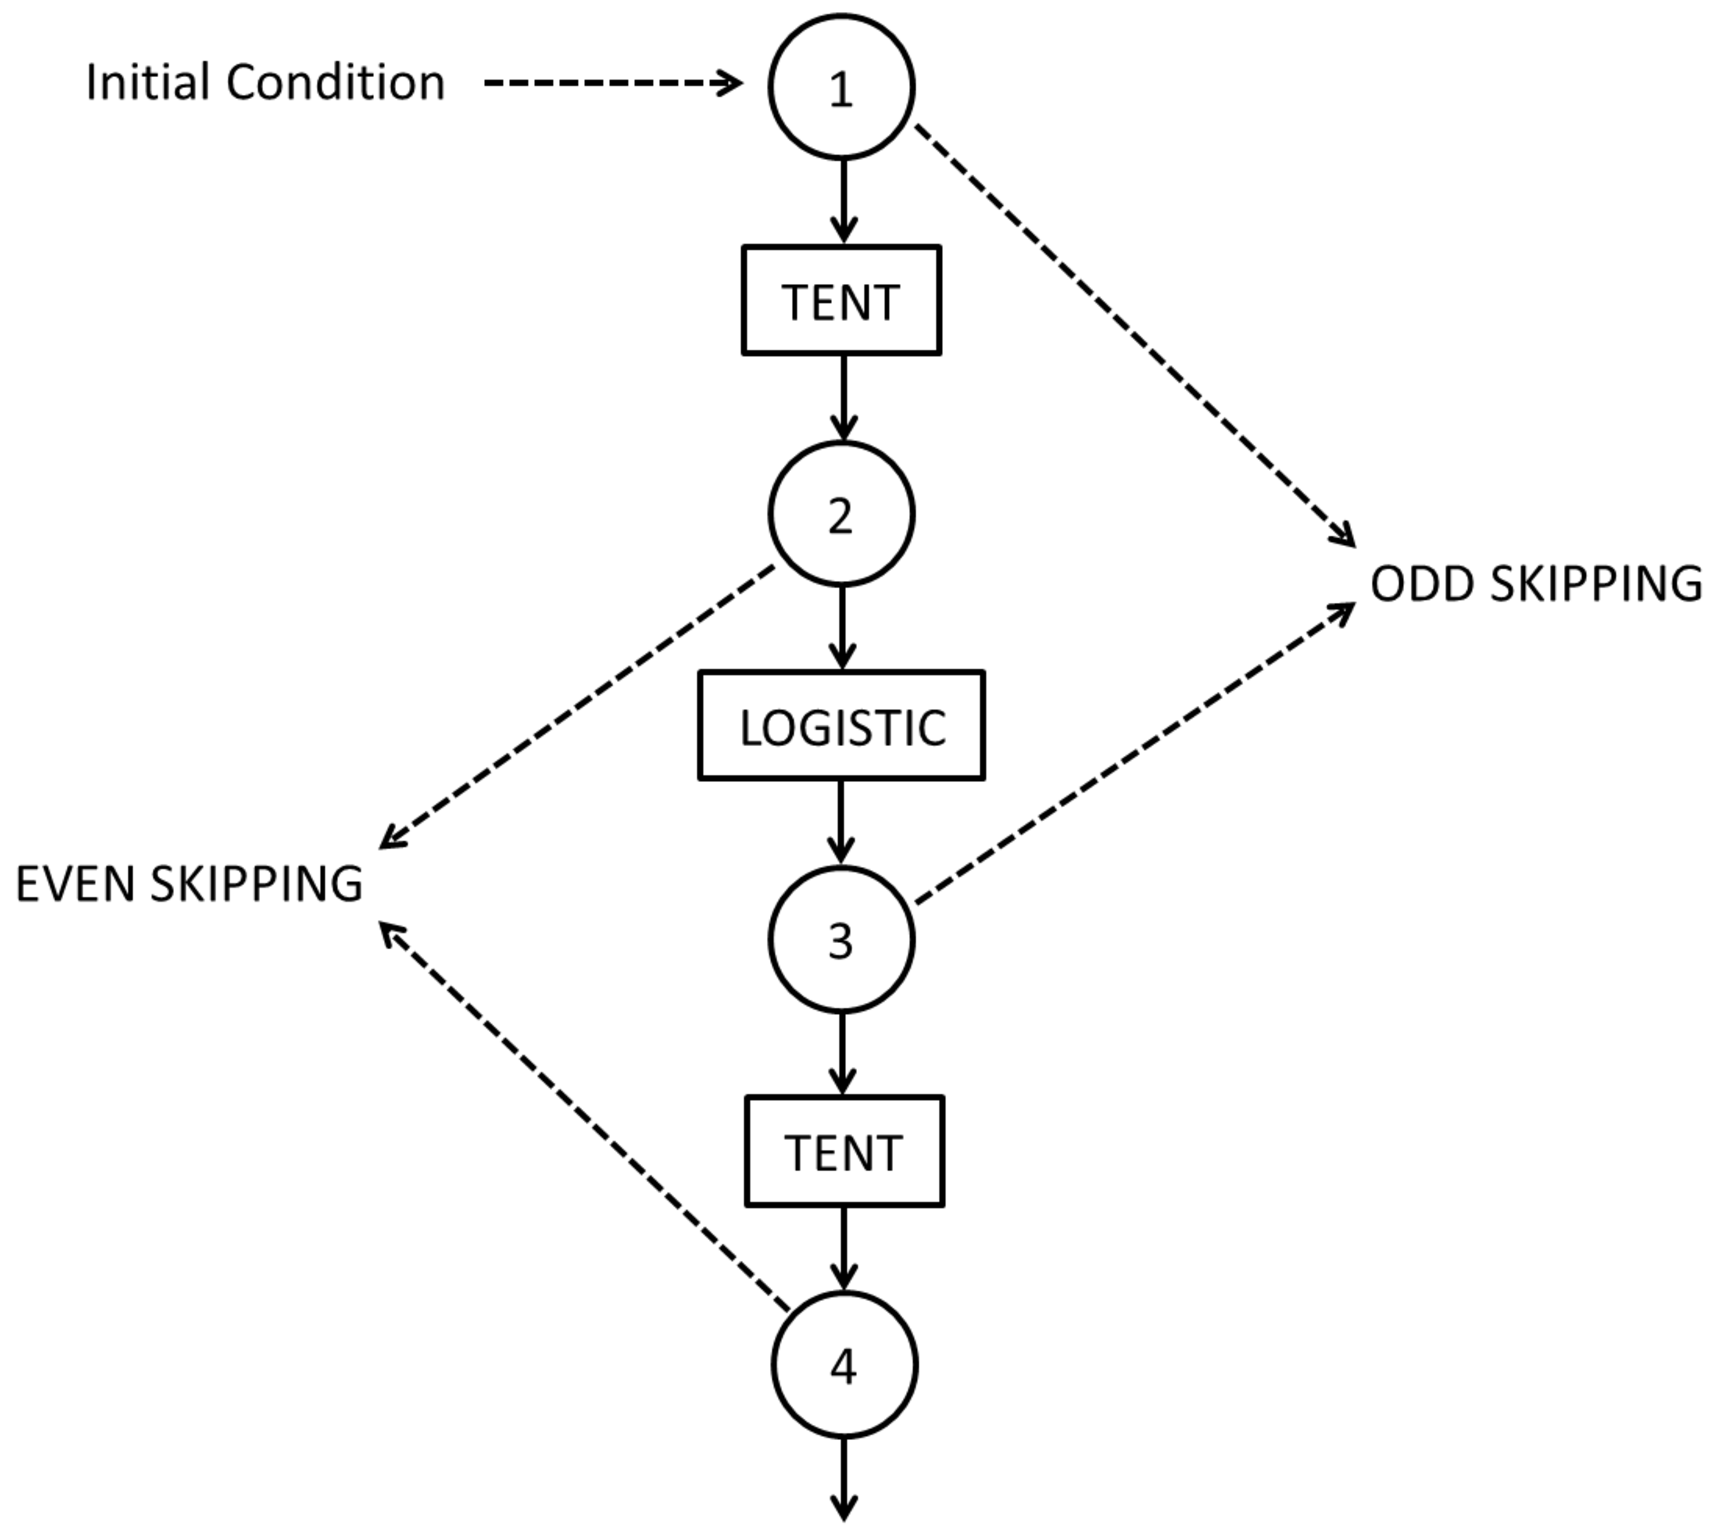
\includegraphics[height=0.4\textheight]{SwitchParImpar}
	\caption{Conmutación secuencial entre TENT y LOG. En la figura también se muestran las estrategias de skipping par e impar.} \label{fig:seq}
\end{figure}

El mapa SWITCH se expresa como:
%
\begin{equation}
\begin{cases}
x_{n+1}=
\begin{cases}
2\,x_n, &, \mbox{if } 0\leq x_n\leq 1/2 \\
2\,(1-x_n ) &, \mbox{if } 1/2<x_n\leq 1
\end{cases} \\
x_{n+2}=4\,x_{n+1}\,(1-x_{n+1})
\end{cases}\label{eq:SWITCH}
\end{equation}
%
con $x_n \in \mathbb{R}$ y $n$ un número par.

El skipping es una técnica habitual de aleatorización que solo aumenta la calidad de mezcla de un mapa y, por consiguiente, aumenta el valor de $H_{BP}$ y disminuye $C_{BP}$ de la serie temporal.
El skipping no cambia los valores de $H_{hist}$ para los mapas ergódicos porque se evalúan utilizando el PDF no causal (histograma de valores normalizado) \cite{DeMicco2008}.

En el caso bajo consideración, estudiamos saltos pares e impares de la conmutación secuencial de los mapas de tent y de logístico:
\begin{enumerate}
	\item Skipping par de la conmutación secuencial de mapas Tent y Logístico (EVEN). \\
	Si $\{x_n; n = 1, \dots, \infty \}$ es la serie de tiempo generada por la eq. \ref{eq: SWITCH}, descarta todos los valores en posiciones impares y conserva los valores en posiciones pares.
	\item Skipping impar de la conmutación secuencial de mapas Tent y Logístico.
	Si $\{x_n; n = 1, \ dots, \ infty \}$ es la serie de tiempo generada por la eq. \ref{eq: SWITCH}, descarta todos los valores en posiciones pares y conserva todos los valores en posiciones impares.
\end{enumerate}

El skipping par se puede expresar como la función de composición TENT $\circ$ LOG mientras que el skipping impar se puede expresar como LOG $\circ$ TENT.
La evolución del período como función de la precisión para estos mapas se informó en \cite{Nagaraj2008}.

Los resultados para cada uno de estos mapas son los siguientes.